For the tighter solid interval, the 32 incident fields have eleven positive generalized source directions, exactly the number required by corollary~\ref{cor:energy}. In units of the incident intensity of one original beam summed over the full square, the infimum in \eqref{eq:energy} is in $[0.59082793,0.59082795]$ at the disk error radius and $[3.74429999,3.74430008]$ at the ring radius. The wider solid interval has thirteen negative material directions and only six positive dictionary directions. The corresponding uniform cap of four has eleven and six. Unlimited fluence in the same dictionary therefore leaves deficits of at least seven and five, respectively. This statement is independent of a particular old receiving record and is specific to its fixed spatial weight. No feed-network power calibration is assumed.

We tested this energy threshold with an occupied class (figure~\ref{fig:nativebeam}). Fix eleven exposures, the same per-column error allowance $r/\sqrt{11}$, and exactly $1.25 E_{\rm inf}$ incident fluence ($0.738535$ in these units). The plane-wave design takes eleven separated dictionary angles; the coherent design uses the leading generalized eigenbeams. Both see the same solid material, the same port geometry and the same normalized noise realization. Saturation holds for both. The coherent design makes $R_y$ positive definite ($\lambda_{\min}>0.00266$), while the angular design leaves five negative receiving directions. This is a strict difference in bounded prediction under one material form at equal incident energy.

The wider solid class was also tested with a physical material in its interior. With 16 and 32 ordinary beams, $\nu=k_o=13$ in both cases; direct evaluation gives 25 positive and seven negative receiving directions in both. This example has enough sources by count and a strictly compatible full-wave solution. Its deficit is the shortage of positive dictionary directions in \eqref{eq:indexsmall}. The narrower and wider tests shared one simultaneous 32-right-hand-side physical solve. Including validated spectral and receiving calculations, the narrow comparison took 78.75 s and the additional wide comparison 38.10 s.

\begin{figure}[tb]\centering
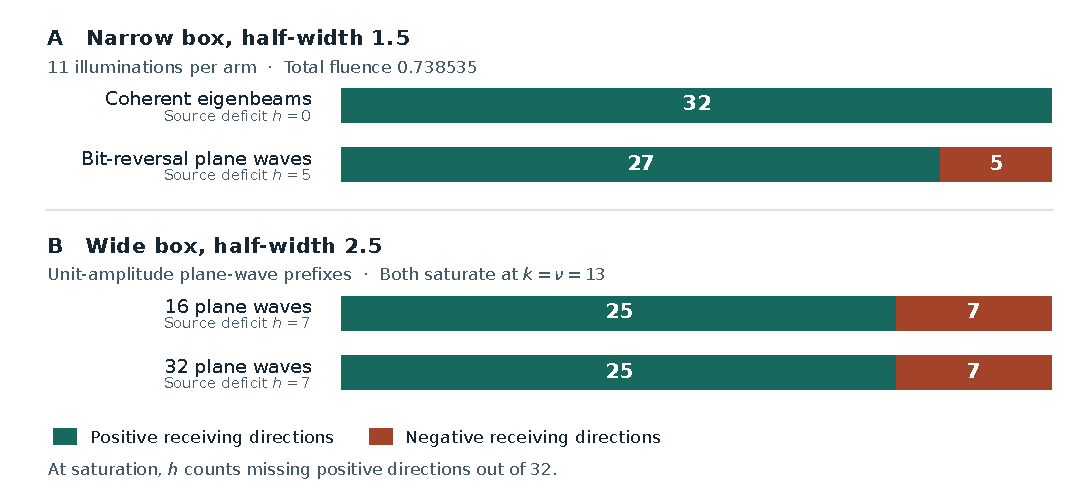
\includegraphics[width=.91\linewidth]{native-illumination}
\caption{Receiving directions on an occupied native material class. Left, identical fluence and eleven exposures per design. Right, nested ordinary-angle prefixes for the wider interval. In both panels a nonpositive receiving direction is a limit of the chosen bound on the scattered response.}\label{fig:nativebeam}
\end{figure}
